\documentclass[a4paper,twoside]{article}

\usepackage{epsfig}
\usepackage{subcaption}
\usepackage{calc}
\usepackage{amssymb}
\usepackage{amstext}
\usepackage{amsmath}
\usepackage{amsthm}
\usepackage{multicol}
\usepackage{pslatex}
\usepackage{algorithm2e}
\usepackage[bottom]{footmisc}
% Please add other packages that you may need BEFORE the SCITEPRESS.sty package.
\usepackage{natbib}
\usepackage{multirow}
\usepackage{SCITEPRESS}

\begin{document}

\title{
  Examining Programming Students’ Interaction with Generative AI: A
  Metacognitive Perspective
}

\author{\authorname{Rodrigo Prestes Machado\sup{1}\orcidAuthor{0000-0003-0428-6387},
Carlos Alario Hoyos\sup{2}\orcidAuthor{0000-0002-3082-0814},
Patricia Callejo Pinardo\sup{2}\orcidAuthor{0000-0001-6124-6213},
Iria Estévez-Ayres\sup{2}\orcidAuthor{0000-0002-1047-5398},
Carlos Delgado Kloos\sup{2}\orcidAuthor{0000-0003-4093-3705}}
\affiliation{\sup{1}Department of Informatics, Instituto Federal de Educação,
Ciência e Tecnologia, Porto Alegre, Brazil}
\affiliation{\sup{2}Department of Telematics Engineering, Universidad Carlos III
de Madrid, Leganés (Madrid), Spain}
\email{\ rodrigo.prestes@poa.ifrs.edu.br, \{calario,pcallejo, ayres,cdk\}@it.uc3m.es}
}

\keywords{
  Programming Education, Generative Artificial Intelligence, Chatbots and
  Metacognition
}

\abstract{
This study examines the interactions of programming students with a chatbot,
CharlieBot, powered by OpenAI's GPT-3.5 and enhanced with the
Retrieval-Augmented Generation (RAG) technique, within the context of a Java
programming course. It investigates how students use the bot while employing two
metacognitive strategies: interleaving and spacing. Using the logs of student
interactions with the bot, the methodology involved classifying and analyzing
student prompts into eight distinct categories. The findings reveal that while
most interactions emphasize active learning strategies, students demonstrate
limited conscious application of interleaving and spacing. This study
underscores the necessity for increased guidance on the strategic use of AI
tools to enhance learning outcomes.
}

\twocolumn\maketitle\normalsize\setcounter{footnote}{0}

\section{\uppercase{Introduction}}
\label{sec:introduction}

Recent advancements in Generative Artificial Intelligence (GenAI) have created
new opportunities in both professional programming \citep{Peng23}
\citep{Pandey24} and education \citep{Puryear22}. In programming courses,
students can employ GenAI tools to enhance their understanding, receive
personalized feedback, and access detailed explanations. For example, GitHub
Copilot, a tool that is integrated into development environments, assists by
providing real-time suggestions and accelerating code writing, which could help
streamline the learning process \citep{Denny23}. Educational chatbots, on the
other hand, try to guide students through coding challenges, answer questions,
and attempt to foster a deeper comprehension of programming concepts
\citep{Labadze23}.

The study guided by \cite{chan23} revealed that both undergraduate and
postgraduate students exhibit positive attitudes towards the use of GenAI in
teaching and learning, noting that it may improve the depth of their thinking
and understanding. Furthermore, a systematic review conducted by \cite{Lo24}
demonstrated that students could effectively learn from ChatGPT, leading to
improved understanding and academic achievement \citep{Callejo24}. Besides that,
it was also observed that ChatGPT enables students to regulate their learning
pace \citep{Baha24} and can potentially support students’ self-regulated
learning, especially for those with previous technical and disciplinary
knowledge \citep{Xia23}.

However, researchers are concerned about the impact of these tools on
students. The systematic review conducted by \cite{Murillo23} indicated that
the use of ChatGPT could lead to an overreliance on the tool. \cite{chan23} also
noted that this dependency could result in a decrease in critical thinking, as
students could make decisions based solely on the information provided by
ChatGPT.

The student’s confidence is justified, as demonstrated by \cite{Puryear22}, who
found that GitHub Copilot can generate solutions for student assignments with
accuracy rates ranging from 68\% to 95\%. However, this also raises concerns
that students may become overly dependent on GenAI tools, potentially bypassing
the opportunity to develop a deeper understanding of the underlying concepts.
\cite{cai23} further highlighted the overdependence and diminished intellectual
engagement as significant drawbacks associated with the use of ChatGPT in
learning.

Regardless of teachers' preferences or beliefs, preliminary surveys conducted
by \cite{Dickey24} revealed that at least 54.5\% of students are already using
GenAI for homework. This highlights the need to increase the understanding of
how students interact with these tools and how they can be used to
enhance learning. Furthermore, a review organized by \cite{Lo24} emphasized the
need for extended studies and objective measures to gather more robust
evidence on the use of GenAI tools in education.

In response to the growing need for deeper insights into the use of GenAI tools
in educational settings, this study aims to help address this gap by analyzing
the interactions between students in a Java programming course and an
educational bot powered by gpt-3.5 from OpenAI, enhanced with
Retrieval-Augmented Generation (RAG) technique. Specifically, it focuses on
examining these interactions within the context of the metacognitive strategies
employed by the students. To achieve this objective, we formulate three research
questions:

\begin{itemize}
  \item RQ1 - What was the distribution pattern of the classified messages?
  \item RQ2 - Was there a space between the student prompts? If so, which
  category promotes the largest spacing between submissions?
  \item RQ3 - Do students' conversations with the bot alternate between
  practical and theoretical approaches, thereby promoting interleaving?
\end{itemize}

% % What is its main limitation?

It is important to consider how GenAI tools impact students in
various demographic groups, academic disciplines, cultural backgrounds, and
levels of previous experience \citep{catalan21} \citep{neo22}. Consequently,
this study is limited to a specific group of students and focuses on the use of
a single GenAI tool. As a result, the findings may not be generalizable to other
populations or tools.

This paper is organized as follows: Section 2 presents the theoretical
framework, Section 3 describes the material and methods used in the study,
Section 4 presents the results and discussion, and Section 5 concludes the
paper and outlines future work.

%% Are there any existing solutions?
% To deal with this issue, some researchers have proposed different pedagogical
% strategies \cite{Denny24} introduced the concept of \textit{Prompt
% Problems}, where students solve programming exercises by formulating natural
% language prompts. \cite{Prasad24} proposed a self-regulated learning framework
% using GenAI to solve programming problems. \cite{Lauren23} explored the
% integration of GenAI with evidence-based learning strategies in computer science
% and engineering courses.

%% Which is the best?

% The study of effective educational strategies in use of GenAI tools in education
% context are important for determining the best training for educators. However,
% as these tools gain popularity among students \cite{Dickey24} the urgency to
% equip educators with best practices may lag behind their rapid adoption.
% Therefore, analyzing students' interaction patterns with GenAI tools is
% important for understanding how these tools are being used and how educators can
% leverage them to enhance learning. In addition, these interaction patterns can
% create new opportunities to redesign GenAI tools to better support pedagogical
% strategies without repressing the development of abstract, critical and creative
% thinking.

\section{\uppercase{Theoretical Framework}}

This section presents the theoretical framework that underpins the study. First,
we introduce the concept of metacognition used in this study. Next, we discuss
related work that explores the use of metacognitive strategies and scaffolds
in educational settings.

\begin{table*}[htbp]
  \caption{Categories - adapted from \cite{Ghimire24}}
  \begin{center}
    \renewcommand{\arraystretch}{1.6} % Increase the spacing between rows
    \begin{tabular}{p{3cm} p{12cm}} % Remove vertical bars
      \hline
      \textbf{Category} & \textbf{Description} \\
      \hline
      Debugging Help & Prompts that seek help to identify, fix errors, or understand the provided code snippet. \\
      Conceptual Question & Prompts that are more about understanding concepts than specific code. \\
      Student Correction & Prompts where the student corrects the bot. \\
      Code Snippet & Prompts that ask for a specific part of the code, like a function or a segment. \\
      Complete Solution & Prompts that request an entire solution or a complete code snippet. \\
      Multiple Question & Prompts where the user wants to solve a multiple choice exercise (Quiz). \\
      Language Change & Prompts that request a change of idiom. \\
      Uncategorized & Prompts that do not fit into any of the above categories. \\
      \hline
    \end{tabular}
    \label{tab:categories}
  \end{center}
\end{table*}

\subsection{Metacognition}

Given that generative AI often produces automatic and highly accurate responses
\citep{Puryear22}, it is essential for students to use these tools within an
active learning process to enhance their learning outcomes. This active
learning process can be further understood through the lens of Metacognition, which
focuses on the awareness of one’s mental processes. \cite{flavell79} proposed a
model of metacognitive monitoring that includes four interrelated phenomena:
Metacognitive Knowledge, Metacognitive Experience, Metacognitive Goals, and
Metacognitive Actions. These processes do not occur in isolation, but they
influence each other, altering cognitive progress over time.

Metacognitive knowledge includes beliefs about variables that affect the
outcomes of cognitive activities. It is divided into three types: beliefs about
personal abilities, perceived difficulty in the task, and previously used
strategies. Metacognitive Experience refers to the feelings that arise
before, during, and after cognitive activity, such as frustration, confusion,
and satisfaction, among others. Metacognitive Goals are the key to regulating
thought as they relate to the goals the individual seeks to achieve, directly
influencing the actions taken. For example, if a student’s goal is to complete
a task quickly, they may adopt a more passive approach to learning. Lastly,
Metacognitive Actions involve the planning, monitoring, and evaluation of
strategies used to achieve the goals. In terms of planning, students can
determine how to approach a task, such as spacing their study sessions
\citep{Ouhao18, Carvalho20}, interleaving topics \citep{Rivers21}, utilizing
retrieval practice \citep{larsen18}, and other strategies.

Spacing and interleaving are two metacognitive strategies that have been shown to
enhance learning outcomes. Spacing refers to the practice of distributing study
sessions over time, which has been shown to improve long-term retention and
understanding of the material \citep{Carvalho20}. Interleaving involves mixing
different topics or problems within a single learning session, which has been
shown to enhance long-term learning and the application of knowledge in other
situations \citep{Rivers21}.

\subsection{Related Work}

Studies on the use of metacognitive strategies indicate that these practices can
be applied to teaching the conscious use of generative AI. \cite{Zheng19}
investigated the effects of metacognitive scaffolds on group behavior,
performance, and cognitive load in computer-supported collaborative
environments. The results showed positive impacts on metacognitive
behavior and group performance without increasing cognitive load.

\cite{LiWei23} proposed a metacognition-based collaborative approach to enhance
performance in collaborative programming. The findings indicated that this
approach influenced computational thinking, critical thinking, and
metacognitive awareness.

Similarly, \cite{Wang23} explored how metacognitive instruction affects
computational thinking, critical thinking, and metacognitive skills in
collaborative programming, observing improvements in problem-solving and
collaboration.

These studies demonstrate the relevance of metacognition in enhancing
performance and skills in collaborative environments without imposing additional
cognitive load. Based on this, it is possible to suggest that metacognitive
strategies may also be useful in teaching a more conscious and critical use of
generative AI tools.

\section{\uppercase{Material and Method}}

This section outlines the tools and procedures used in this study. CharlieBot
served as the GenAI tool for educational purposes, and the method was structured
into three distinct phases, each designed to systematically assess its
interaction with students.

\subsection{CharlieBot}

CharlieBot is an educational bot built on ChatGPT 3.5 and enhanced with
Retrieval-Augmented Generation (RAG) technique to improve the precision of
responses provided to students \cite{Sun24}. The RAG feature was developed using
materials from a MOOC, including text, exercises, video transcripts, and other
resources.

\subsection{Method}

The study was conducted in three phases: data collection,
categorization, and analysis. During the data collection phase, students
enrolled in a second semester Java course at a public university in Spain were
introduced to CharlieBot and allowed to use it freely, without being subjected
to a specific methodology for its use. Data were collected anonymously, ensuring
that the records of interactions could not be linked to any individual student
or their academic performance.

In the categorization phase, the students' messages were manually classified
into eight distinct categories for analysis. Initially, \cite{Ghimire24}
proposed four categories: Debugging Help, Conceptual Question, Code Snippet,
and Complete Solution. However, the data collected indicated the need for
additional categories, leading to the inclusion of four more: Multiple Choice
(Quiz), Student Corrections, Language Change, and Uncategorized. In this study,
students were free to use the bot as they wanted, which contributed to the
emergence of these additional categories. Table \ref{tab:categories} presents
these categories along with their respective descriptions.

The analysis phase involved the use of Python scripts to extract information
from previously classified data. The datasets and code snippets used in this
process are available at: YYY.

\section{\uppercase{Results and Discussion}}

A total of 343 student messages were categorized in 42 conversations, with
an average of 8.17 messages per conversation. This data offers insights into how
users engage with CharlieBot and the types of prompts they submit. The results of
the analysis are presented in this section, addressing the research questions
outlined in the introduction.

Figure \ref{fig:graph1} shows the distribution of the messages in the
categories:

\begin{figure}[h!]
    \centering
    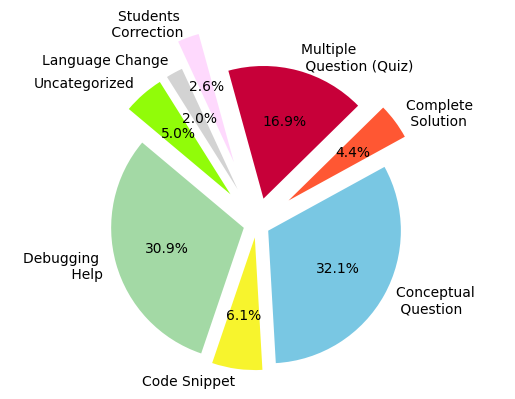
\includegraphics[scale=0.62]{img/figure1.png}
    \caption{Classification of messages.}
    \label{fig:graph1}
\end{figure}

\begin{figure*}[htbp]
  \centering
  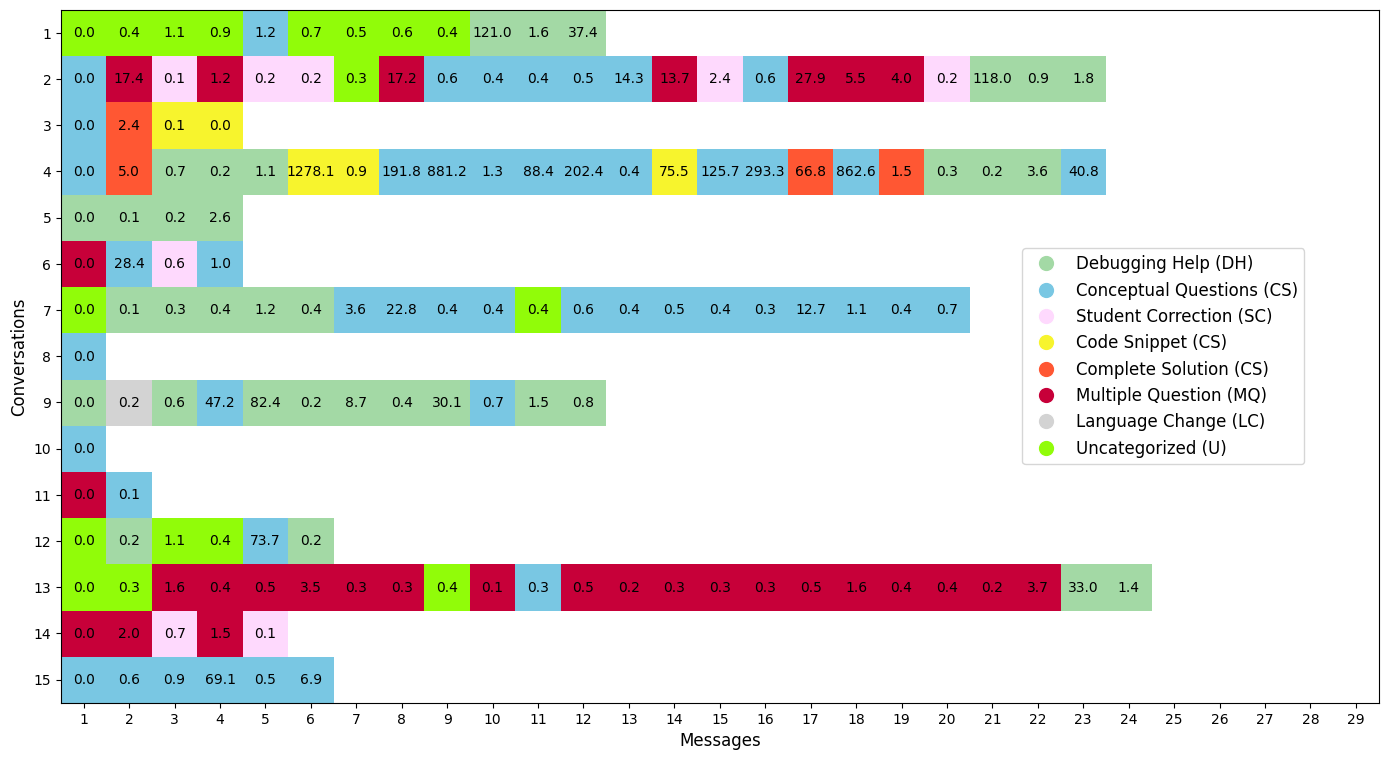
\includegraphics[scale=0.52]{img/figure2.png}
  \caption{Examples of conversations.}
  \label{fig:graph2}
\end{figure*}

\subsection{Classification of Messages}

About the first research question: \textit{What was the distribution pattern of
the classified messages?}

According to Figure \ref{fig:graph1} messages classified as
Conceptual Question account for 32.1\% of the total. Often, the sequence of
Conceptual Question begins with a request for a Complete Solution or Code
Snippet, which then evolves into a series of Conceptual Question, as seen in
conversation 2 of Figure \ref{fig:graph2}. In other cases, the conversation
consists entirely of messages classified as Conceptual Question, such as in
conversation 10 of Figure \ref{fig:graph2}. This type of message indicates that
students recognize that they have not yet fully mastered a concept and are seeking to
better understand it. In this context, the student realizes that solving the
problem requires understanding of concepts, thus applying an active learning
strategy.

As shown in Figure \ref{fig:graph1}, approximately 30.9\% of the messages were
classified as Debugging Help. These prompts often begin with a request for a
Complete Solution or Code Snippet. Following this, students typically switch from
passive to more active learning strategy, as illustrated by the start
of conversation 12 in Figure \ref{fig:graph2}. Debugging Help messages represent
a form of active learning, in which students likely focus on gaining a practical
understanding of the code, identifying errors, and improving their debugging
skills for future tasks.

Since most of the messages are located in categories where students are
notoriously engaged in being more active in their learning (Conceptual Question
and Debugging Help), corroborating the findings of \cite{Ghimire24} which
showed that the questions are also localized in the same categories.

Requests for the bot to generate a Code Snippet or Complete Solution accounted
for 10.5\% of student messages. These prompts reflected a desire for more
direct answers; however, it was observed that, after receiving these solutions,
many students transitioned to a more active approach in seeking to understand
the code or the underlying concepts. Thus, it can be inferred that the prompts
within the Code Snippet or Complete Solution category were often used as a
starting point for a more in-depth study.

Multiple Choice exercise resolutions represented 16.9\% of the responses.
These prompts typically involved students submitting one or more exercises to
CharlieBot and requesting solutions. We identified sequences of multiple choice
questions, as illustrated by conversations 8, 9, and 15 in \ref{fig:graph2}.
This less active learning approach can occur for various reasons, ranging from
the belief that reviewing solutions to similar questions enhances learning, to
issues such as negligence, poor planning, or other possible factors.

Student corrections to bot responses accounted for 2.6\% of the
interactions. In most cases, these corrections occurred when the student already
had the correct answer to an exercise and identified an error in the bot
response, as illustrated in conversations 4 and 9 in Figure \ref{fig:graph2}.
These corrections highlight that, although the bot provides quick feedback, it
is not always accurate and its errors can be difficult for students to
identify.

Figure \ref{fig:graph1} also shows that around 5\% of the prompts written by
students were not categorized. These messages range from greetings to the Bot,
such as a simple "\textit{Hola}," to contextual statements like
"\textit{Estoy repasando orientación a objetos.}"

\subsection{Spacing}

% Spacing

About the second research question: \textit{Was there a space between the student
prompts? If so, which category promotes the largest spacing between
submissions?}

Spacing, a well-established learning strategy \citep{Carvalho20}, was analyzed
by examining the time intervals between user interactions with CharlieBot.
Approximately 26.2\% of the conversations, or roughly a quarter, included pauses
longer than 60 minutes. However, this data only indicates that students paused
their use of the AI, which could suggest that they were either reflecting on the
topic independently or engaging in unrelated activities. Furthermore, 16.7\%
of the conversations exhibited pauses of 12 hours and 9\% showed delays
exceeding 24 hours between messages, indicating that some degree of spacing
occurred. However, it is important to note that this behavior may have been
influenced by the design of the initial version of CharlieBot, which only kept
the chat session active as long as the student kept the browser tab open and
avoided reloading the page. This adds uncertainty about the precise context in
which students applied spacing.

There is a noticeable difference in the interaction time with the bot when a
student asks a conceptual question. This was probably due to the fact that, in
this category, the student is more focused on understanding a concept and
engaging in deeper learning, which aligns with the metacognitive goal of
promoting comprehension and long-term retention. Figure \ref{fig:graph3}
shows the average interaction time per category.

\begin{figure*}[htbp]
  \centering
  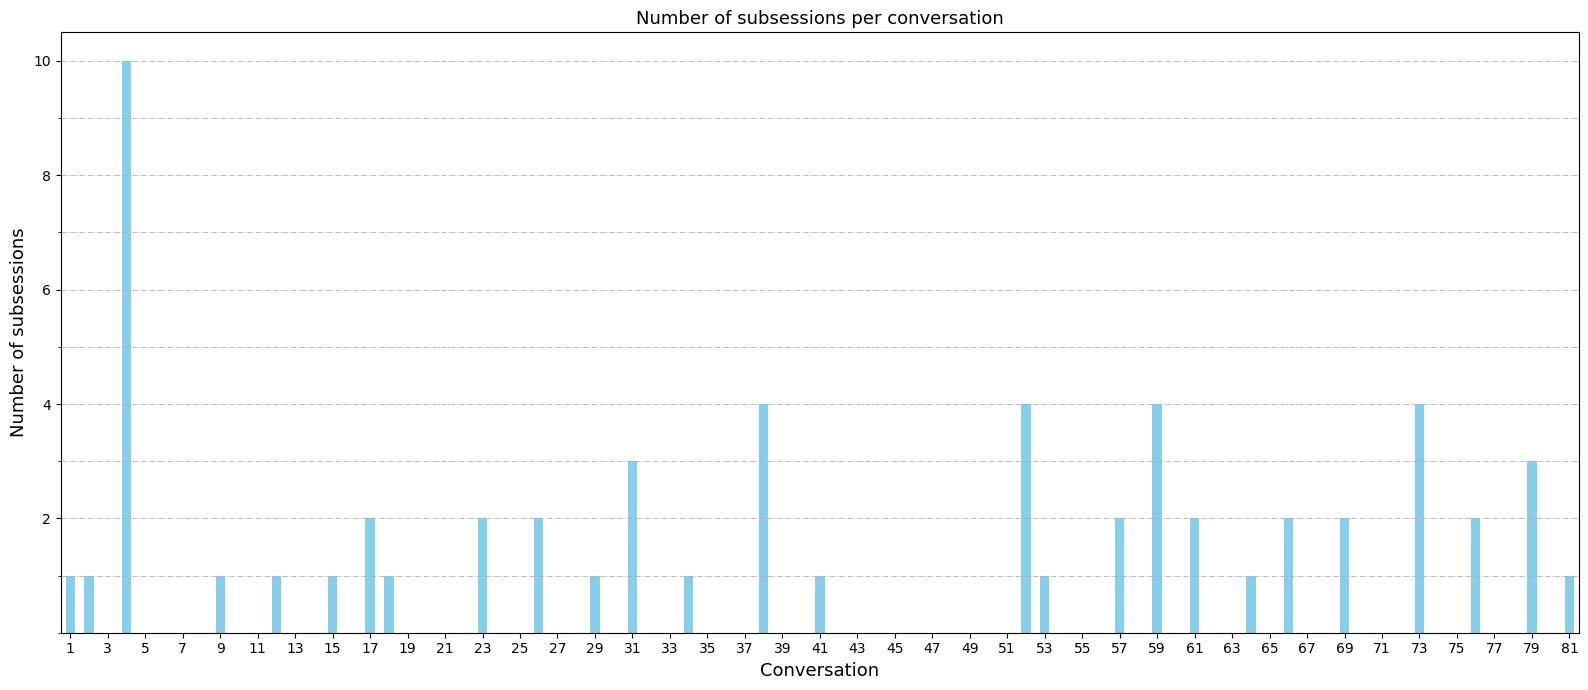
\includegraphics[scale=0.55]{img/figure3.png}
  \caption{Average interaction time per category.}
  \label{fig:graph3}
\end{figure*}

\subsection{Interleaving}

% Interleaving

Regarding the third research question: \textit{Do students' conversations with
the bot alternate between practical and theoretical approaches, thereby
promoting interleaving?}

Intervealing is a learning strategy that involves mixing or alternating
different topics or problems within a single learning session. This approach has
been shown to be useful for promoting long-term learning and improving the
application of knowledge in other situations \citep{Rivers21}.

When analyzing the classification of messages in conversations, we identified
the presence of sequences of messages belonging to the same category, which
could suggest a low occurrence of interleaving. To illustrate the presence of
blocks, Figure \ref{fig:graph2} presents examples of conversations and their
classification. In Conversation 2, the student alternates messages among Code
Snippet, Debugging Help, and Conceptual Question, showing a tendency to
interleave from a practical to theoretical perspective. In contrast, in
Conversation 10, the student focused on a single block of Conceptual Question.
Although the focus was on understanding a theoretical concept, this conversation
tended not to promote interleaving, due to the absence of alternation between
different types of task.

To better assess the extent of these sequences, we calculated the percentage of
messages that were part of repeated blocks. Considering blocks with at least
three messages, we observed that 56.2\% of the student's prompts were grouped
into some sequence. When analyzing blocks with a minimum of four messages, we
found that 47.5\% of the prompts were part of continuous sequences.

However, if we consider that sequential messages from a certain point indicate
that the student is \textit{blocked} (or focused) on a task, the remaining space
for interleaving is 43.8\%, assuming a block starting from at least three
consecutive messages, and 52.5\% for blocks starting from four consecutive
messages. Thus, the data suggest that interleaving occurs on students'
conversations with CharlieBot, but in which situations and with what type of
student profile is a study that needs to be further investigated.

\section{Conclusion and Future Work}

TODO: Work in progress.

* The results indicate that most interactions are focused on active learning
strategies, although deliberate use of interleaving and spacing is limited. We
believe that students can be guided to adopt a more deliberate approach in
utilizing GenAI, enabling them to more effectively harness these tools to
enhance their learning.

* Due to the anonymity of the interactions, it's unclear whether
students were intentionally using interleaving and spacing strategies or if
these patterns emerged naturally. Future research should investigate whether
students were consciously applying.

* To provide teachers with valuable data for analyzing how students are using
the tools, we are developing an AI model to automatically classify student
messages. This will enable educators to better understand student behavior and
offer more targeted support where needed.

\section*{ACKNOWLEDGEMENTS}

The authors would like to thank the Federal Institute of Education, Science and
Technology (IFRS) for the partial financial support provided for the execution
of this research.

\bibliographystyle{apalike}
{\small
\bibliography{References}}

\section*{\uppercase{\textit{Appendix}}}

If any, the appendix should appear directly after the
references without numbering, and not on a new page. To do so please use the
following command: \textit{$\backslash$section*\{APPENDIX\}}

\end{document}


% % Conceptual Question
% \subsubsection*{Sequence of Conceptual Question}

% Messages classified as conceptual question represent around 32\% of all
% messages. We have found a pattern of sequences of Conceptual Question in some
% conversations. Some conversations are entirely composed of messages classified
% as Conceptual Question. In other cases, the sequence of Conceptual question
% starts with a request for a Complete Solution or a Code Snippet, followed by
% a progression of Conceptual Question. In both cases, the student is actively
% engaging with the bot to understand the concepts and compromised with more
% deep learning.

% Regarding Metacognitive Knowledge, these sequences of prompts classified as
% Conceptual Question, can be interpreted that the students are aware they have
% not fully mastered a concept and are trying to understand it, demonstrating a
% good level of self-awareness. In this sense, the student realizes that the
% problem requires an understanding of concepts in order to advance in their
% studies. In this way, the student applies an active learning strategy.

% About Metacognitive Experience, several types of feelings may be associated at
% this moment, such as actively reflecting on the answers, uncertainty and/or
% confusion when trying to understand the concept, frustration for not
% progressing, and satisfaction as their questions are answered in a way that
% facilitates understanding.

% Regarding the type of Metacognition related to objective of the Task, the
% students may recognize the difficult and trying to achieve a deeper
% understanding of the evolved concepts to later apply in practice.

% With respect to Metacognitive Strategies, the student demonstrates a sence of
% planning to identify their knowledge gaps. They may start with more general
% questions to obtain an overview of the concept and then ask more specific
% questions as they gain more clarity. Because the questions are in sequence, the
% student probably can adequately monitor their progress.

% % Multiple Choice
% \subsubsection*{Sequence of Multiple Choice}

% Around 16.9\% of the messages were classified as Multiple Choice. These prompts
% typically involve students sending one or more exercises to CharlieBot, asking
% for the solution.

% We identified a sequence of Multiple Choice patterns in some of the
% conversations. From the point of view of Metacognitive Knowledge, a possible
% interpretation of this complex phenomenon is that students may believe in their
% inability to answer several questions. They may also assume that the questions
% share a common theme, and solving them together may help consolidate knowledge.
% Additionally, they might understand that obtaining the answers quickly is more
% efficient.

% Regarding Metacognitive Experiences, students may experience feelings such as
% cognitive overload, a sense of urgency, and/or confidence in ready-made answers,
% which can often lead to relief and a reduction of frustration.

% Concerning the Metacognitive about the Task, one interpretation may be that the
% student simply wants to complete the task quickly to alleviate the workload,
% and/or obtain a correct answer without focusing on deeper learning at
% this moment.

% In relation to Metacognitive Strategies, students are likely focusing on saving
% time and/or possibly lacking planning skills. They may also perceive that
% solving the questions on their own requires too much cognitive effort, but this
% pattern might reveal a lack of progress monitoring and understanding of
% concepts. After obtaining the answers, the metacognitive evaluation process
% could lead to feelings of satisfaction, but further reflection may indicate that
% the strategy was not effective in supporting deep learning. Depending on this
% evaluation, it may influence future decision-making to change the strategy.

% % Debugging help
% \subsubsection*{Sequence of Debugging Help}

% Around 30.9\% of the messages were classified as Debugging Help. Besides of
% that, we identified a pattern of a sequences of Debugging Help in the
% conversations. These prompts typically start with a message requesting a
% Complete Solution or a Code Snippet. After that, the students normally chance
% from passive to more active learning strategy.

% In terms of Metacognitive Knowledge, the student probably recognizes that they
% do not have the necessary tools or knowledge to debug the code on their own.
% Concerning the understanding of the task, they may know that debugging is not
% just a matter of superficial corrections but requires understanding the
% underlying logic. Thus, the student apparently believes that the sequence of
% questions related to debugging will help them understand the codes.

% In terms of Metacognitive Experiences, some feelings may arise at this moment,
% such as frustration or uncertainty in the face of errors, confusion during the
% process, and also growing confidence or satisfaction as they better understand
% the code and possible corrections.

% With respect to Metacognitive related with the objective of the Task, the
% student is probably focused on understanding the code in practical terms,
% identifying errors, and learning how to better debug in the future.

% As for Metacognitive associated with the Strategy, the student has requested
% external help and realizes that dividing the debugging task into several
% questions can result in a better understanding of the code. They can monitor
% their progress throughout the process, adjusting their questions as necessary,
% evaluate the effectiveness of the responses received, and reflect on what was
% learned during the process.
